\documentclass{beamer}


\usepackage{listings}


\let\solution\relax
\let\endsolution\relax


\usepackage{gvv}


\usepackage[utf8]{inputenc}
\usepackage{lmodern}
\usepackage{xcolor}
\usepackage{graphicx}
\usepackage{amsmath,amssymb}


\lstset{
	language=C,
	basicstyle=\ttfamily\small,
	keywordstyle=\color{blue},
	commentstyle=\color{green},
	stringstyle=\color{red},
	breaklines=true,
	breakatwhitespace=true,
	showstringspaces=false,
	frame=single,
	morekeywords={import, as, from, ctypes, numpy, matplotlib, pyplot, None},
	xleftmargin=0pt,
	framexleftmargin=0pt,
	aboveskip=0pt,
	belowskip=0pt
}



\definecolor{myblue}{RGB}{48, 63, 159}
\setbeamercolor{palette primary}{bg=myblue, fg=white}
\setbeamercolor{structure}{fg=myblue}
\setbeamercolor{frametitle}{bg=myblue, fg=white}
\setbeamercolor{title}{bg=myblue, fg=white}
\setbeamercolor{footlinecolor}{bg=myblue, fg=white}

\title{2.5.16}
\author{Shriyansh Chawda-EE25BTECH11052}
\date{August 23, 2025}

\begin{document}
	
	\setbeamertemplate{footline}{} 
	\frame{\titlepage}
	
	\begin{frame}{Question} 
		Find the value of $p$ for which the lines
		\[
		\frac{1-x}{3} = \frac{2y-14}{2p} = \frac{z-3}{2} 
		\quad \text{and} \quad 
		\frac{1-x}{3p} = \frac{y-5}{1} = \frac{6-z}{5} 
		\]
		are perpendicular. 
		\hfill (12, 2019)
	\end{frame}
	
	\begin{frame}{Solution}
		Writing each line in symmetric form to read off direction vectors:
		\begin{align}
			\vec{x} &= \vec{A} + \lambda \vec{m}
		\end{align}
		
		From
		\begin{align}
			\frac{1-x}{3}=t,\;
			\frac{2y-14}{2p}=t,\;
			\frac{z-3}{2}=t,
		\end{align}
		we obtain
		\begin{align}
			x = 1-3t,\quad
			y = 7+pt,\quad
			z = 3+2t.
		\end{align}
		
		Hence,
	\begin{align}
		\vec{m_1} = \myvec{-3 \\ p \\ 2}
	\end{align}
	\end{frame}
	
	\begin{frame}{Solution}
		From
		\begin{align}
			\frac{1-x}{3p}=s,\;
			\frac{y-5}{1}=s,\;
			\frac{6-z}{5}=s,
		\end{align}
		we obtain
		\begin{align}
			x = 1-3ps,\quad
			y = 5+s,\quad
			z = 6-5s.
		\end{align}
		
		Hence,
\begin{align}
		\vec{m_2} = \myvec{-3p \\ 1 \\ -5}
\end{align}
	\end{frame}
	
	\begin{frame}{Solution}
		The lines are perpendicular when
		\begin{align}
			\vec{m_1}^\top \vec{m_2} &= 0
		\end{align}
		Substituting,
		\begin{align}
			\myvec{-3 & p & 2}\myvec{-3p\\[2pt] 1\\[2pt] -5} &= 0 \\
			(-3)(-3p) + p\cdot 1 + 2(-5) &= 0 \\
			9p + p - 10 &= 0 \\
			10p - 10 &= 0 \\
			\Longrightarrow\; p &= 1
		\end{align}
		
		Therefore,
		\[
		\boxed{p=1}
		\]
	\end{frame}
	\begin{frame}
\begin{figure}[h!]
	\centering
	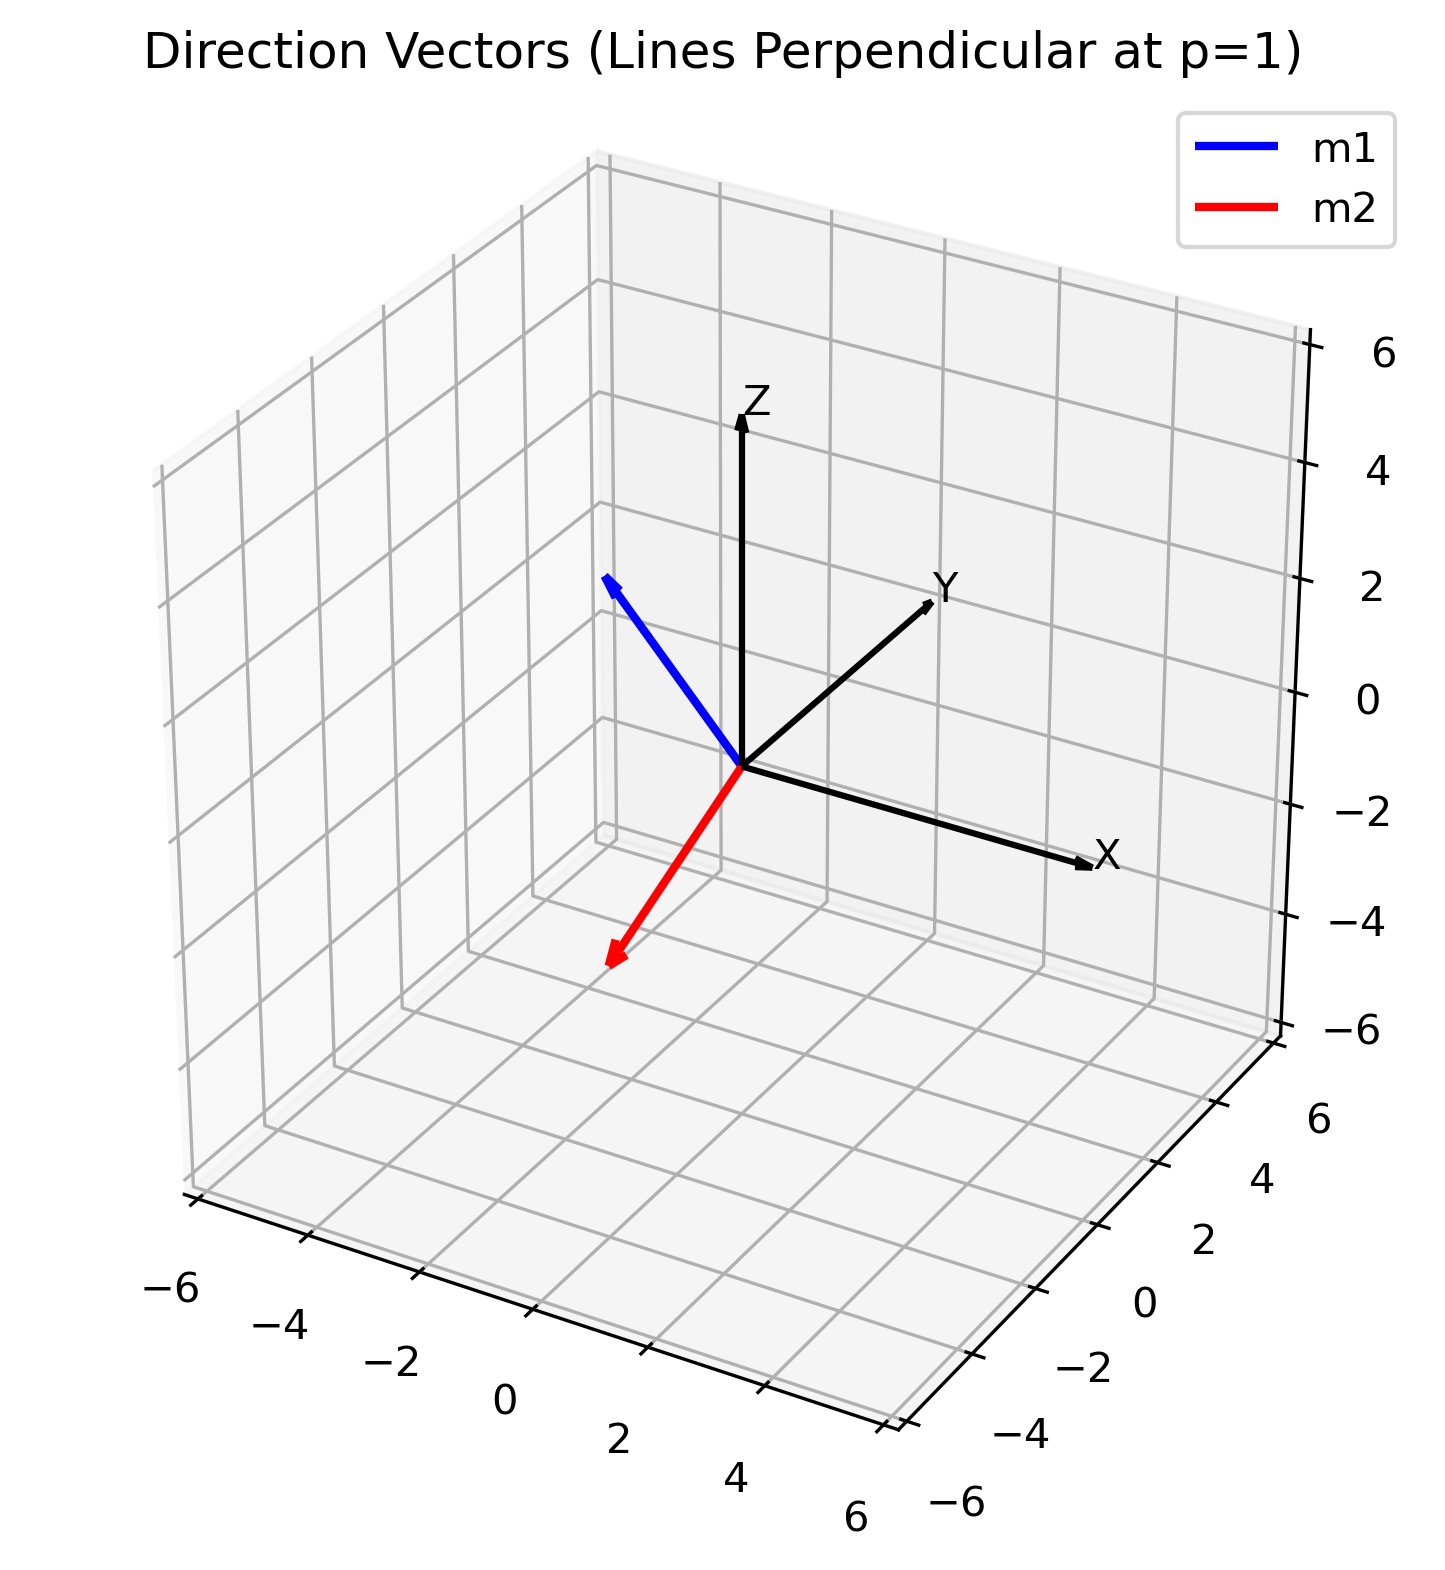
\includegraphics[width=0.7\linewidth]{figs/equations_solution}
	\caption{Plotting both lines}
	\label{fig:equationssolution}
\end{figure}

	\end{frame}
	
\end{document}
